\documentclass[titlepage=firstcover, captions=tableheading]{scrartcl}
\usepackage{microtype}
\usepackage{amsmath}
\usepackage{polyglossia}
\usepackage{graphicx}
\usepackage{booktabs}
\usepackage{siunitx}
\usepackage{hyperref}
\usepackage{caption}
\usepackage{float}
\setdefaultlanguage{german}
\title{311 Der Hall-Effekt}
\author{
Connor Magnus Böckmann \\ email: \href{mailto:connormagnus.boeckmann@tu-dortmund.de}{connormagnus.boeckmann@tu-dortmund.de}
\and Tim Theissel \\ email: \href{mailto:tim.theissel@tu-dortmund.de}{tim.theissel@tu-dortmund.de}  
}
\begin{document}
\maketitle
\newpage
\tableofcontents
\newpage
\section{Zielsetzung}
Das Ziel des Versuchs 311 "Hall-Effekt und Elektrizitätsleitung bei Metallen" ist die Ermittlung der Leitfähigkeit einer Metallprobe anhand makroskopisch messbarer Parameter, wie etwa den geometrischen Abmessungen, der Hallspannung und dem Widerstand.

\section{Theoretische Grundlagen}
\subsection{Bandstruktur und Leitfähigkeit von Kristallen}
Kristalle bestehen aus Gittern, in denen die Atome so nah beieinander sind, dass sich ihre Valenzelektronen-die Außenelektronen-sich verhalten wie ein kontinuirliches System. Alle diese Elektronen unterliegen jedoch dem Pauli-Prinzip, welches besagt, dass keine zwei Elektronen im exakt gleichen Quantenzustand sein können. Das führt dazu, dass alle Elektronen unterschiedliche Energien besitzen. Im Unterschied zu den streng definierten Energieniveaus eines Einzelatoms, bilden sich hier also quasi kontinuierliche Energiebänder. Die Lücke zwischen zwei Energiebändern nennt man dabei verbotene Zone. Diese Energien können also nicht von Elektronen angenommen werden. Die Energiebänder können nur eine endliche Anzahl von Elektronen enthalten. Aufgefüllt werden die Energiebänder immer von den unteren Orbitalen zu den oberen Orbitalen. Elektronen aus vollbesetzten Bändern tragen nicht zur Leitfähigkeit bei, da sie keine Energie durch ein elektrisches Feld aufnehmen können. Ungepaarte Elektronen in nicht voll besetzten Energiebändern können sich in Richtung eines angelegten elektrischen Feldes bewegen. Ein makroskopischer elektrischer Strom entsteht. Die hohe elektrische Leitfähigkeit von Metallen resultiert also aus ihren nur teilweise besetzten oberen Energiebändern. Dieses wird Leitfähigkeitsband genannt. \\
Bei Isolatoren ist das oberste Energieband folglich leer und die verbotene Zone zu breit, um von Elektronen aus einem niedrigeren Band übersprungen zu werden. \\
Ein ideales Kristallgitter müsste nach der Quantentheorie eine unendlich hohe elektrische Leitfähigkeit besitzen, was aber auf Grund von Gitterbaufehlern nicht der Fall ist.
\subsection{Zur Berechnung der elektrischen Leitfähigkeit eines Metalles}
Die Leitungselektronen eines Metalls verhalten sich wie die Teilchen eines idealen Gases und stoßen beständig mit Strukturfehlern und Ionenrümpfen zusammen. Man kann nun die Zeit zwischen zwei Zusammenstößen mitteln und so die mittlere Flugzeit $\bar{\tau}$ erhalten. Wenn nun ein elektrisches Feld anliegt, werden die Elektronen während $\bar{\tau}$ gleichmäßig beschleunigt. Die Geschwindigkeitsänderung beträgt dann:
\begin{equation}
   \Delta \vec{\bar{v}}=-\frac{e_0}{m_0}\vec{E}\bar{\tau}
\end{equation}
Das Elektron wird dabei in eine zufällige Richtung gestreut. Im Mittel hat es also bei Beginn der Flugzeit die Geschwindigkeit 0 in Richtung des elektrischen Feldes. Daher kann eine mittlere Driftgeschwindigkeit $\vec{\bar{v_d}}$ eingeführt werden:
\begin{equation}
    \vec{\bar{v_d}}=\frac{1}{2}\Delta\vec{\bar{v}}
\end{equation}
Wenn nun ein elektrischer Leiter n Elektronen pro Volumeneinheit enthält und sich diese mit $\vec{\bar{v_d}}$ in Richtung von $\vec{E}$ bewegen, ist die Stromdichte j:
\begin{equation}
    j=-n\bar{v_d}e_0
\end{equation}
Dabei kann man $\bar{v_d}$ durch (?) und (?) ausdrücken.
\begin{equation}
    j=\frac{1}{2}\frac{e_0^2}{m_0}n\bar{\tau}E
\end{equation}
Es wird ein homogener Leiter (Länge L und Querschnitt Q) angenommen, weshalb j durch I/Q und E durch U/L ersetzt werden können.
\begin{equation}
    I=\frac{1}{2}\frac{e_o^2}{m_0}n\bar{\tau}\frac{Q}{L}U
\end{equation}
Der hier dargestellte Proportionalitätsfaktor zwischen der Spannung und Strom ist die elektrische Leitfähigkeit S:
\begin{equation}
    S=\frac{1}{2}\frac{e_o^2}{m_0}n\bar{\tau}\frac{Q}{L}
\end{equation}
Das Reziproke zur Leitfähigkeit ist der elektrische Widerstand R:
\begin{equation}
    R=2\frac{m_0}{e_0^2}\frac{1}{n\bar{\tau}}\frac{L}{Q}
\end{equation}
Daraus ergeben sich die geometrieunabhängigen Werte der spezifischen Leitfähigkeit \sigma und des spezifischen Widerstands\rho:
\begin{equation}
    \sigma=\frac{1}{2}\frac{e_o^2}{m_0}n\bar{\tau}
\end{equation}

\begin{equation}
    \rho=2\frac{m_0}{e_0^2}\frac{1}{n\bar{\tau}}
\end{equation}
Der Widerstand lässt sich leicht und relativ präzise an einem Draht messen. Die Gleichung enthält aber weiterhin mikroskopische Größen-n und $\bar{\tau}$. Daher werden weitere Zusammenhänge zwischen mikroskopischen Größen und makroskopisch messbaren Parametern benötigt.

\subsection{Der Hall-Effekt}
Im folgenden wird sich auf den in Abb.2 gezeigten Versuchsaufbau bezogen und die Bezeichnungen daraus verwendet. \\
\begin{figure}[H]
    \centering
    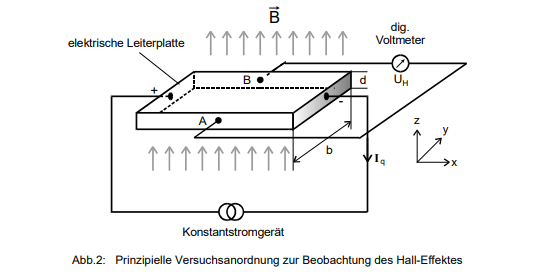
\includegraphics[height=9cm]{Versuchsanordnung_HallEffekt.png}
    \captionbelow{Abb.2: Prinzipielle Versuchsanordnung zur Beobachtung des Hall-Effektes}
\end{figure}
An eine homogene Leiterplatte, die Probe, der Dicke d und der Breite b wird der Länge nach ein konstanter Strom I\textsubscript{q} angelegt. An den Punkten A und B kann dann eine so genannte Hallspannung gemessen werden, wenn dann die Probe noch senkrecht zur Stromrichtung von I\textsubscript{q} von einem homogenen Magnetfeld $\vec{B}$ durchsetzt wird. Diese entsteht auf Grund der Lorentzkraft $\vec{F\textsubscript{L}}$, welche auf die Elektronen wirkt und diese ablenkt.
\begin{equation}
    F_L=e_0\vec{\bar{v_d}}B
\end{equation}
Sie zeigt dabei in negative y-Richtung wegen der negativen Ladung der Elektronen. Dadurch erhalten die Elektronen eine Geschwindigkeit in y-Richtung, woduch ein weiteres E-Feld entsteht, welches als $\vec{E\textsubscript{y}}$ der Bewegung in y-Richtung entgegen wirkt. $\vec{E\textsubscript{y}}$ wird dabei genau so groß, dass es die Lorentzkraft aufhebt.
\begin{equation}
    e_0E_y=e_0\vec{\bar{v_d}}B
\end{equation}
Die Hallspannung berechnet sich dann zu:
\begin{equation}
    U_H=E_y*b=\vec{\bar{v_d}}B*b
\end{equation}
$\vec{\bar{v_d}}$ lässt sich dabei durch den Querstrom I\textsubscript{q}:
\begin{equation}
    j=\frac{I_q}{b*d}=-ne_0\vec{\bar{v_d}}
\end{equation}
Also gilt:
\begin{equation}
    U_H=-\frac{1}{ne_0}\frac{B*I_q}{d}
\end{equation}
Die benötigte Ladungsträgerdichte n errechnet sich also nach:
\begin{equation}
    n=-\frac{1}{U_He_0}\frac{B*I_q}{d}
\end{equation}
Mit bekanntem n lässt sich nun die mittlere Flugzeit $\bar{\tau}$ berechnen:
\begin{equation}
    \bar{\tau}=2\frac{m_0}{e_0^2}\frac{1}{nR}\frac{L}{Q}
\end{equation}
Außerdem lässt sich $\vec{\bar{v_d}}$ nun bestimmen:
\begin{equation}
    \vec{\bar{v_d}}=\frac{I}{-nQe_0}
\end{equation}
\subsection{Weitere Leitfähigkeitsparameter aus R und U\textsubscript{H}}
Der nächste zu bestimmende Parameter ist die mittlere freie Weglänge $\bar{l}$. Sie stellt die Entfernung, die ein Leitungselektron im Mittel zwischen zwei Zusammenstößen im Kristall zurücklegt. Sie errechnet sich nach:
\begin{equation}
    \bar{l}=\bar{\tau}*\mid v\mid
\end{equation}
\mid v\mid stellt dabei die Totalgeschwindigkeit der Elektronen dar. Da diese, wie bereits oben beschrieben wurde, dem Pauli-Verbot unterliegen, gilt nicht die klassische Maxwell-Boltzmann-Statistik. Viel mehr lässt sich zeigen, dass Elektronen der Fermi-Dirac-Verteilung unterliegen:
\begin{equation}
    f(E)=\frac{1}{e^\frac{E*E_F}{kT}+1}dE
\end{equation}
Die Fermi-Energie E\textsubscript{F} errechnet sich zu:
\begin{equation}
    E_F=\frac{h^2}{2m_0}\sqrt[3]{(\frac{3}{8\pi}n)^2}
\end{equation}
h stellt dabei das Planksche Wirkungsquantum dar. Im Wesentlichen hängt E\textsubscript{F} von der Dichte der Elektronen im Festkörper ab. Nur die wenigen Elektronen mit E\approx E\textsubscript{F} sind verantwortlich für die Leitfähigkeit des Metalls, da diese Energie aus einem äußeren E-Feldes aufnehmen können. Daraus folgt für $\mid \bar{v} \mid$:
\begin{equation}
    \mid \bar{v} \mid\approx \sqrt{\frac{2E_F}{m_0}}
\end{equation}
Für die gesuchte freie Weglänge ergibt sich daraus:
\begin{equation}
    \bar{l}\approx\bar{\tau}\sqrt{\frac{2E_F}{m_0}}
\end{equation}
Außerdem lässt sich die mikroskopische Größe der Beweglichkeit \my der Ladungsträger bestimmen. Sie ist definiert als Verhältnis zwischen Driftgeschwindigkeit $\vec{\bar{v_d}}$ und der äußeren Feldstärke.
\begin{equation}
    \vec{\bar{v_d}}=\my\vec{E}
\end{equation}
\begin{equation}
    \my=\frac{1}{2}\frac{e_0}{m_0}*\bar{\tau}
\end{equation}
\subsection{Elektrizitätsleitung bei Metallen mit positiven Ladungsträgern}
Bei zweiwertigen Metallen kommt es gelegentlich vor, dass die Energiebänder der Elektronen sich überlappen, wodurch die Elektronen spontan vom unteren ins obere Band springen können. Da sie nun im unteren Band fehlen, hinterlassen sie dort Fehlstellen, so genannte Löcher. Diese Löcher können sich unter dem Einfluss eines äußeren E-Feldes bewegen. Sie sind also nicht ortsfest und wirken wie eine positive Ladung. Der Hall-Effekt der durch sie erzeugt wird nennt sich anomaler Hall-Effekt. Durch die umgekehrte Ladung dreht sich bei der Hall-Spannung das Vorzeichen. Somit lässt sich am Vorzeichen erkennen, ob die Löcher oder die Leitelektronen dominant zur Leitfähigkeit beitragen. Erst bei Materialien in denen Löcherleitung und Elektronenleitung in etwa gleichem Maße vorliegen, wird die Unterscheidung anhand dieses Kriteriums quasi unmöglich. 
\end{document}